\subparagraph{Predication Example 1: }
Consider the following code sequence.

\begin{verbatim}

00	r2 <- r1 op r0
10	b_op r2, 030
20	r3 <- r1 op r0
30	r4 <- r1 op r0

\end{verbatim}

This example illustrates a simple minimal control dependency
situation.
Instruction 30 does not depend, either through a data flow dependency
or a control flow dependency, on any of the instructions that
are shown to be before it.  The branch instruction 10 is data
dependent on instruction 00 (through register
{\tt r2}.
Instruction 20 is control
dependent on instruction 10 (the branch).
The branch is initially predicted to be not-taken.
The execution sequence of this example is shown
in Figure
Figure~\ref{pex1}.

\begin{figure}
\centering
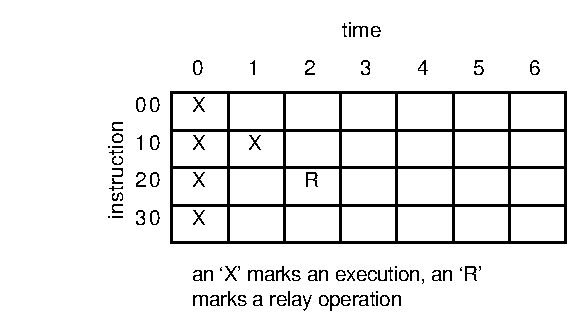
\epsfig{file=pex1.eps,height=1.50in}
\caption{{\em Timing of the code example, predication scenario 1.}
This example illustrates the exploitation of basic minimal control
dependencies, a significant contribution to
achieving higher ILP by taking advantage of independent
instructions beyond the joins of branches.
Execution of an instruction at a given time is
again indicated by an `X'.}
\label{pex1}
\end{figure}


We start by assuming that all instructions execute in a single clock
cycle and that they all execute immediately upon being loaded.
It is assumed that the initial execution of the branch in
instruction 10 (at time 0) did not change its predicate output.
However, since instruction 00 executed in clock cycle 0, we will
assume that its output value changed from what was originally loaded
at instruction load time.  Instruction 00 will broadcast forward
its new updated output (register
{\tt r2}).
Since instruction 10 (the branch) is data dependent on
register
{\tt r2}
from instruction 00, it will snoop for that update
and snarf the new value from the forward broadcast.  
This will enable it to re-execute.
We assume that it executes at the earliest possible time.
This would be clock cycle 1.  On this execution, its output predicate,
essentially its branch prediction, does change.  The branch may either
have been resolved at this point or simply may have made a new prediction
based on a possibly still speculative value of register
{\tt r2}.
A change in the branch condition will change its
predication output and this will be
broadcast out.
If the branch became resolved and a DEE path originating due to this
branch had been started, an implementation may abandon the
current main-line execution path and switch the DEE path of this branch
to become the new main-line path.
For this example, we will assume that
no switch to a DEE paths occurs.  When no switch to a DEE path occurs,
instruction 20, being control dependent on the branch, will be snooping
for the branch predicate change and seeing that it has changed
will switch to relaying its output value.  
The relay operation
takes the value for register
{\tt r3} that was loaded, or snarfed, from before the execution
of instruction 20, and re-broadcasts it.  The re-broadcast of the relayed 
output value is necessary in those cases where following instructions
used the previously broadcasted output value.
The relaying operation would have
also occurred
if a DEE path became the new main-line path
but implementations can choose to switch executions paths or
not as an optimization.

In spite of the branch being predicted one way and then changed
to the other (whether re-predicted or resolved), it should be
noted that instruction 30 was not required to be re-executed as
a result.  This illustrates a basic minimal control dependency
which serves to facilitate higher instruction level parallelism (ILP)
by taking advantage of independent instructions located beyond the
joins of branch domains.

